\tikzset{
  clase/.style={draw, thick},
  nombre/.style={font=\small},
}

\begin{enumerate}
  \item Hay un único diagrama posible:

  \begin{center}
  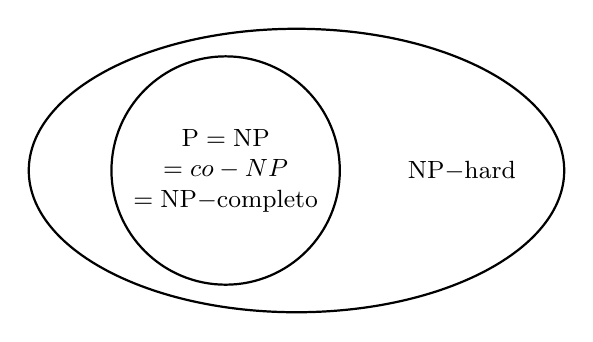
\begin{tikzpicture}
    \draw[clase] (0.9, 0) ellipse (3.4 and 1.8);
    \node[nombre] at (3.0, 0) {\(\mathrm{NP\text{-}hard}\)};
    \draw[clase] (0, 0) circle (1.45);
    \node[nombre, align=center] at (0, 0) {\(\mathrm{P} = \mathrm{NP}\)\\\(= \text{co-NP}\)\\\(= \mathrm{NP\text{-}completo}\)};
  \end{tikzpicture}
  \end{center}

  \begin{itemize}
    \item \(\mathrm{P} = \text{co-P}\) siempre es cierto (¡lo demostramos en clase!).
    \item \(\mathrm{P} = \mathrm{NP}\) implica que \(\text{co-NP} = \mathrm{NP}\) (también lo demostramos). 
    \item \(\mathrm{NP\text{-}hard}\) contiene problemas que no son \(\mathrm{NP}\) (e.g., el \textit{halting problem}).
  \end{itemize}


  \item No hay ningún diagrama posible. Demostramos en clase que \(\mathrm{P} \subseteq \mathrm{NP} \cap \text{co-NP}\) y sabemos que \(\mathrm{P}\) no es vacío (porque si fuera vacío, entonces ¿qué hicimos las primeras 8 semanas del curso?)

  \item Hay un único diagrama posible:

  \begin{center}
  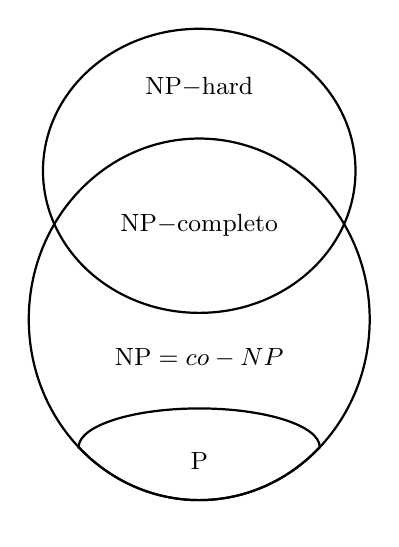
\begin{tikzpicture}[scale=0.82, font=\small, thick]
    \draw (0, -1.0) ellipse (2.640 and 2.8);
    \node at (0, -1.6) {\(\mathrm{NP} = \text{co-NP}\)};

    \draw (0, 1.3) ellipse (2.420 and 2.2);
    \node at (0, 2.6) {\(\mathrm{NP\text{-}hard}\)};

    \node at (0, 0.45) {\(\mathrm{NP\text{-}completo}\)};

    % P's bottom arc follows the NP oval, joining it at 225 and 315 degrees.
    \draw (-1.867, -2.980)
      arc[start angle=225, end angle=315, x radius=2.640, y radius=2.8]
      arc[start angle=0, end angle=180, x radius=1.867, y radius=0.6]
      -- cycle;
    \node at (0, -3.2) {\(\mathrm{P}\)};
  \end{tikzpicture}
  \end{center}

  \begin{itemize}
    \item \(\text{co-NP} \cup \mathrm{NP} = \text{co-NP}\) equivale a \(\mathrm{NP} \subseteq \text{co-NP}\), lo cual implica \(\mathrm{NP} = \text{co-NP}\): si \(L \in \text{co-NP}\), entonces \(\overline{L} \in \mathrm{NP} \subseteq \text{co-NP}\), luego \(L \in \mathrm{NP}\).
    \item \(\mathrm{NP\text{-}completo} = \mathrm{NP} \cap \mathrm{NP\text{-}hard}\).
    \item Como \(\mathrm{P} \neq \mathrm{NP}\), ningún problema \(\mathrm{NP\text{-}completo}\) está en \(\mathrm{P}\).
    \item \(\mathrm{NP\text{-}hard}\) contiene problemas que no son \(\mathrm{NP}\) (e.g., el \textit{halting problem}).
  \end{itemize}
\end{enumerate}
